% Headers
\documentclass[a4paper]{article}

\usepackage{tabu}
\usepackage[utf8]{inputenc}
\usepackage[english]{babel}
\usepackage[T1]{fontenc}
\usepackage[margin=3cm]{geometry}
\usepackage{graphicx}
\usepackage{acronym}
\usepackage{marvosym} % Special symbols (e.g. \Letter, \Telefon, \Email)
\usepackage{blindtext} % Very good package for sample text, language specific (use e.g. \usepackage[ngerman]{babel} before). Way better than the lipsum package (for examples see: http://ctan.mirrorcatalogs.com/macros/latex/contrib/blindtext/blindtext.pdf)
\usepackage{caption} % Better captioning (e.g. when clicking on Link to figure, the whole figure is viewable, not only the description)
\usepackage{listings} % Code listings
\usepackage{color} % Use of colors
\usepackage{eurosym}
\usepackage{float}
\usepackage{comment}
\usepackage{booktabs}
\usepackage[table,xcdraw]{xcolor}
\usepackage{pdflscape}

% Project specific stuff
\usepackage{fancyvrb}
\usepackage[nottoc]{tocbibind} % Get bibliography, LOF, LOT and LOL into TOC (Without numbers!). From http://tex.stackexchange.com/questions/71129/bibliography-in-table-of-contents
%\usepackage[nottoc,numbib]{tocbibind} % Bibliography with number  in TOC. See http://tex.stackexchange.com/questions/8458/making-the-bibliography-appear-in-the-table-of-contents
% tocbibind general usage: ftp://ftp.tex.ac.uk/tex-archive/macros/latex/contrib/tocbibind/tocbibind.pdf

\usepackage{newclude} % removes some restrictions from \include (e.g. pagebreak before and after \include). Details: http://ctan.mackichan.com/macros/latex/contrib/frankenstein/newclude.pdf

\definecolor{mygreen}{rgb}{0,0.6,0}
\definecolor{mygray}{rgb}{0.5,0.5,0.5}
\definecolor{mymauve}{rgb}{0.58,0,0.82}
\definecolor{mybeige}{RGB}{255,213,122}

\lstset{ %
    backgroundcolor=\color{mybeige},   % choose the background color; you must add \usepackage{color} or \usepackage{xcolor}
    basicstyle=\footnotesize,        % the size of the fonts that are used for the code
    breakatwhitespace=false,         % sets if automatic breaks should only happen at whitespace
    breaklines=true,                 % sets automatic line breaking
    captionpos=b,                    % sets the caption-position to bottom
    commentstyle=\color{mygreen},    % comment style
    deletekeywords={...},            % if you want to delete keywords from the given language
    escapeinside={\%*}{*)},          % if you want to add LaTeX within your code
    extendedchars=true,              % lets you use non-ASCII characters; for 8-bits encodings only, does not work with UTF-8
    frame=single,                    % adds a frame around the code
    keepspaces=true,                 % keeps spaces in text, useful for keeping indentation of code (possibly needs columns=flexible)
    keywordstyle=\color{black},      % keyword style
    language=Octave,                 % the language of the code
    morekeywords={*,...},            % if you want to add more keywords to the set
    numbers=none,                    % where to put the line-numbers; possible values are (none, left, right)
    numbersep=5pt,                   % how far the line-numbers are from the code
    numberstyle=\tiny\color{mygray}, % the style that is used for the line-numbers
    rulecolor=\color{black},         % if not set, the frame-color may be changed on line-breaks within not-black text (e.g. comments (green here))
    showspaces=false,                % show spaces everywhere adding particular underscores; it overrides 'showstringspaces'
    showstringspaces=false,          % underline spaces within strings only
    showtabs=false,                  % show tabs within strings adding particular underscores
    stepnumber=2,                    % the step between two line-numbers. If it's 1, each line will be numbered
    stringstyle=\color{mymauve},     % string literal style
    tabsize=2,                       % sets default tabsize to 2 spaces
    title=\lstname                   % show the filename of files included with \lstinputlisting; also try caption instead of title
}

% Variables
\newcommand{\titlepageFile}{./titlepage/titlepage-english}
\newcommand{\referencesFile}{./references}
\newcommand{\templateSection}{./sections/template-section}
\newcommand{\exOneSection}{./sections/ex1}
\newcommand{\exTwoSection}{./sections/ex2}
\newcommand{\exThreeSection}{./sections/ex3}
\newcommand{\exFourSection}{./sections/ex4}

% For efficient document generation. Details: http://www.weinelt.de/latex/includeonly.html
\includeonly{
    \titlepageFile,
    \templateSection/template,
    \exOneSection/ex1,
    \exTwoSection/ex2,
    \exThreeSection/ex3,
    \exFourSection/ex4}

% Packages that should be at the end of the preamble

\usepackage[
    backend=bibtex,
    style=authoryear,
    sortlocale=en_EN,
    natbib=true,
    url=true, 
    doi=true,
    eprint=false
]{biblatex}

\usepackage[autostyle]{csquotes}
\addbibresource{\referencesFile}

\usepackage[ % Clickable references
	pdfstartview={FitV},
	pdftitle={CSS SS2015 Assignment 1 -- Group 25},
	pdfauthor={},
	pdfsubject={Compuational Social Simulation},
	colorlinks=false
]{hyperref}
% % % % % % % % % % % % % % % % % % % % % % % % % % % % % % % % %
% % % % % % % % Common variables for titlepages % % % % % % % % %
% % % % % % % % % % % % % % % % % % % % % % % % % % % % % % % % %
\newcommand{\productiondate}{14.04.2015}
\newcommand{\lva}{Workflow Modeling and Proces Management}
\newcommand{\lvanr}{188.924}
\newcommand{\advisor}{Univ.Lektor Dipl.-Ing. Dr.rer.soc.oec. Marco Zapletal}
\newcommand{\advisoremail}{marco.zapletal@tuwien.ac.at}

% Students
\newcommand{\studentAname}{Pavol Loffay}
\newcommand{\studentAmatr}{e1429587}
\newcommand{\studentAmail}{e1429587@student.tuwien.ac.at}

\newcommand{\studentBname}{Ing. Johannes Luef}
\newcommand{\studentBmatr}{e0828182}
\newcommand{\studentBmail}{e0828182@student.tuwien.ac.at}

\newcommand{\studentCname}{Ing. Christian Ohrfandl, BSc}
\newcommand{\studentCmatr}{e0926341}
\newcommand{\studentCmail}{christian.ohrfandl@tuwien.ac.at}

\newcommand{\studentDname}{Fabian Pimminger, BSc}
\newcommand{\studentDmatr}{e1025104}
\newcommand{\studentDmail}{e1025104@student.tuwien.ac.at}

\newcommand{\studentEname}{Thomas Claus Solich, BSc}
\newcommand{\studentEmatr}{e1027433}
\newcommand{\studentEmail}{e1027433@student.tuwien.ac.at}

% % % % % % % % % % % % % % % % % % % % % % % % % % % % % % % % %
% % % % % % % % Custom commands for titlepages  % % % % % % % % %
% % % % % % % % % % % % % % % % % % % % % % % % % % % % % % % % %

% \tabular -- Page-break in a cell. From http://tex.stackexchange.com/questions/2441/how-to-add-a-forced-line-break-inside-a-table-cell
\newcommand{\specialcell}[3][c]{%
    \begin{tabular}[#1]{@{}#2@{}}#3\end{tabular}}
% % % % % % % % % % % % % % % % % % % % % % % % % % % % % % % % %
% % % % % % % % Variables for english titlepage % % % % % % % % %
% % % % % % % % % % % % % % % % % % % % % % % % % % % % % % % % %
\newcommand{\prtypeENG}{}
\newcommand{\prsubjectENG}{Project Proposal}
\newcommand{\prdescriptionENG}{Customer Care Center}
\newcommand{\lvafilltextENG}{written as part of the lecture}
\newcommand{\advisorfilltextENG}{advised by}
\newcommand{\studentfilltextENG}{Group: 04}
\newcommand{\datefilltextENG}{Vienna, }

% Begin of document
\begin{document}

% English titlepage
\include{\titlepageFile}

% TOC
\tableofcontents
\newpage

% Sections
\section{Project description\label{sec:proddesc}}
The goal of this project will be the creation of a program which manages customer requests from different sources. Customers can contact the customer care center via e-mail, Facebook or Twitter. The program automatically polls requests from these sources. Incoming requests are enriched (e.g. with a unique ID) and passed to an agent who processes the request. The customer also immediately receives a confirmation message indicating the customer care center received the request. All requests are logged and there is also a backup process which translates the requests to XML format and syncs it with a Dropbox account. The different EIPs, components and their purposes will be described later on.

\subsection{Features}
\begin{itemize}
    \item receive user ticket requests via different channels (email, Facebook, Twitter)
    \item route ticket requests to different positions (agent, calendar)
    \item append messages to existing tickets
    \item filter spam mails
    \item reply to messages
    \item convert logs to XML and backup via a Dropbox account
\end{itemize}

\subsubsection{EIPs}
\begin{enumerate}
    \item Content Based Router -- Distinguish between message channels (email, Facebook, Twitter)
    \item Message Filter -- will be used to filter spam (based on a blacklist)
    \item Aggregator -- if a ticket is closed the aggregator is used to combine all messages and save them in the database
    \item Splitter -- will be used to separate facebook posts (as they are grouped via polling)
    \item Wire Tap -- will be used to log incoming requests and forward requests to employees at the same time
    \item Message Translator -- will be used to translate requests into a XML format
    \item File Transfer -- take the translated XML-Backup and sync it with a Dropbox account
    \item Logging EIP -- will be used for logging purposes (see wire tap)
    \item Content Enricher -- get Ticket IDs from existing business cases
    \item Seda Queue -- will be used for syncing Twitter tweets
    \item Polling -- will be used to get emails, facebook-posts
\end{enumerate}

\subsubsection{Components (incl. Beans/Processors)}
\begin{enumerate}
    \item Dropbox -- will be used to store backups of the requests (in XML format)
    \item Google calendar -- will be used to store appointments of customer care center employees with customers
    \item Database + camel-mongodb -- will be used to save all exchanged messages with a timestamp
    \item Facebook -- company has a facebook profile which can be used by customers to contact the company
    \item Twitter -- company also has a twitter profile which customers can use to post requests
    \item camel-mail -- besides facebook and twitter customers can also contact the company by mail
    \item camel-velocity -- this component will be used to create auto response templates (e.g. for the response that the request entered the customer care center)
\end{enumerate}

\newpage
\section{Graphical Process Model}
%\begin{lstlisting}
%The proposal has to contain a graphical process model (BPMN 2.0).
%\end{lstlisting}
\begin{figure}[ht!]
	\centering 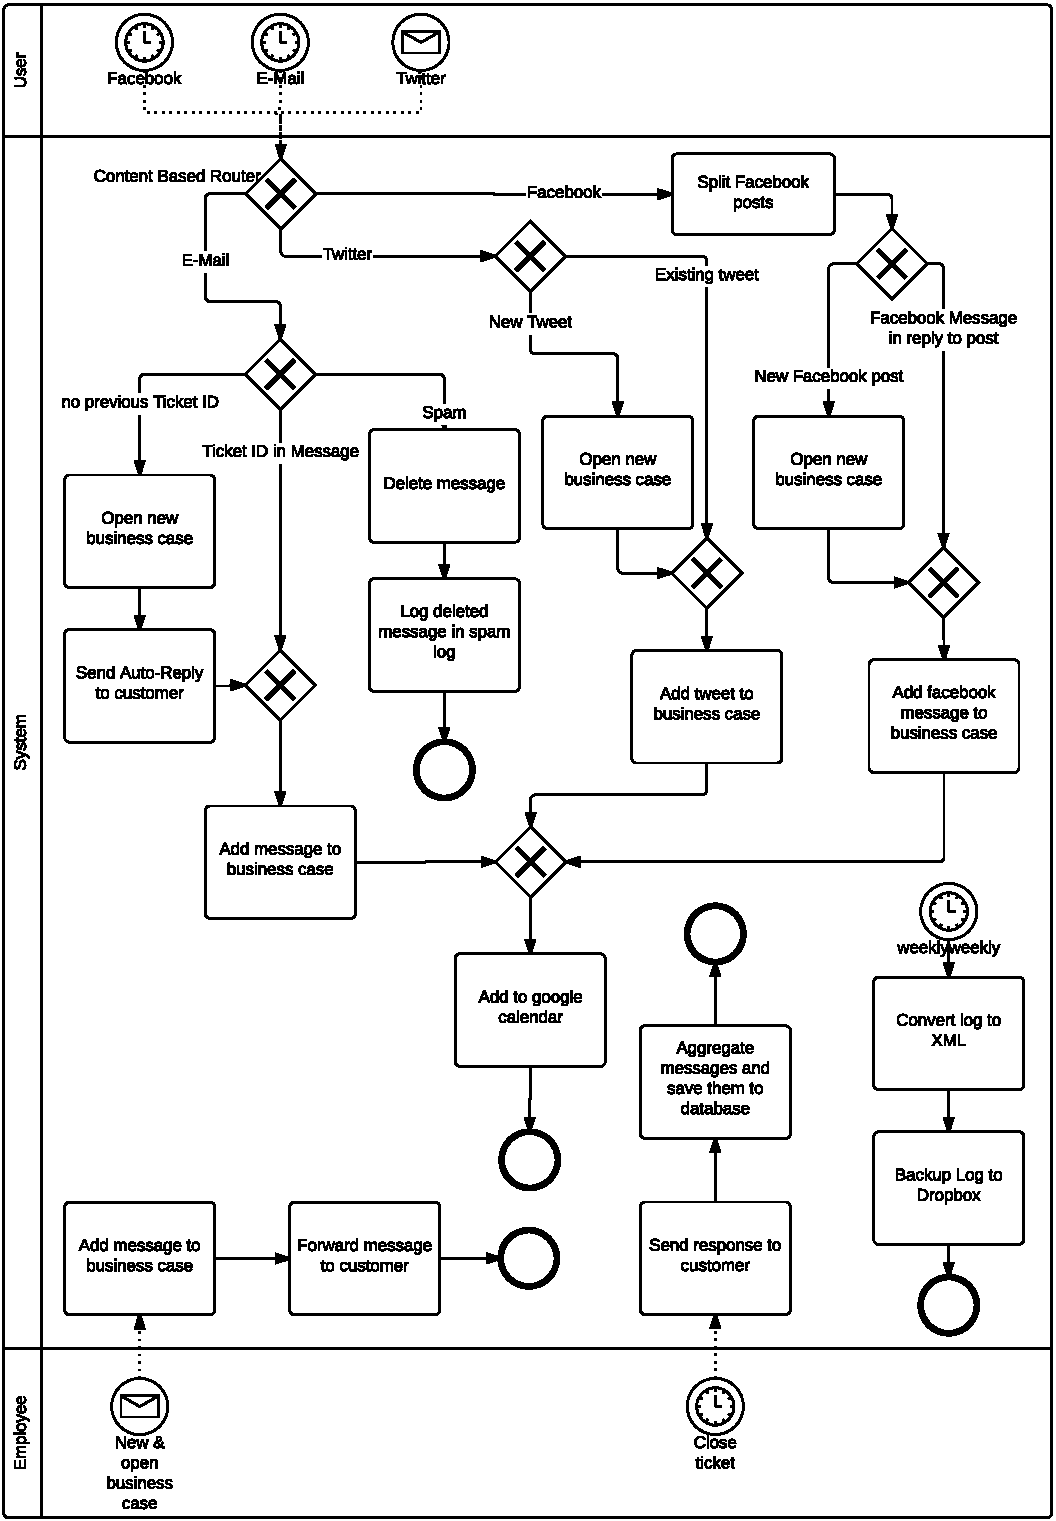
\includegraphics[width=1.00\linewidth]{./media/BPMN-2-0.pdf}
	\caption{BPMN 2.0 Model}
	\label{fig:bpmn}
\end{figure}

\subsection{Description of the graphical process model}
The user can send requests to our helpdesk via Facebook, email or Twitter. Depending on the input channel, a content based router decides which path in the further process the request takes. E-Mails are divided in three categories
\begin{enumerate}
\item New requests: A new business case is opened, an auto-reply with the new ticket-id will be generated and returned to the customer. 
\item New mails for an existing ticket (where the subject contains a ticket-id): If there is an open business case with this ticket number the message will be added to it.
\item Spam (will be filtered, deleted and logged)
\end{enumerate}
In case of a Twitter-request it will be checked if it is a reply to an existing Tweet. In this case the new tweet will be added to the existing business case. Otherwise a new business case will be opened.

For Facebook posts it works similar to Twitter with the only difference that Facebook posts are split (since they are polled). 

The business cases are then saved to a Google calendar (to schedule customer appointments). 
Employees can add messages to business cases and forward them to customers.

On a weekly basis the logs are converted to XML files and saved to a Dropbox folder (as a backup).

\section{Architecture}
\begin{itemize}
    \item Application concentrated on business logic
    \item Use of a MongoDB
    \item Apache Camel for message routing
    \item Dependancy Managment (Maven)
\end{itemize}

\section{Cost estimation\label{sec:costest}}

\begin{table}[H]
\caption{Cost estimation}
\resizebox{\textwidth}{!}{%
\begin{tabular}{@{}llll@{}}   % |l|c|c|}
\toprule
\multicolumn{1}{c}{\textbf{Cost estimation}}           & \textbf{\%}                          & \textbf{hours/member} \\ \toprule
Management (meetings, documents, records, documentation) & 20                                   & 10                    \\ 
Requirement specification                                & 5                                    & 2,5                   \\ 
Design                                                   & 10                                   & 5                    \\ 
Coding                                                   & 30                                   & 15                    \\ 
Testing                                 & 10                                   & 5                    \\ 
System- and Integrationtests                             & 15                                   & 7,5                  \\ 
Overhead(error handling, bug fixing, riskmanagement)     & 10                                   & 5                    \\ \midrule
\textbf{Sum hours/member}                                & \multicolumn{1}{l}{\textbf{100 \%}} & \textbf{50}          \\ 
\textbf{Sum overall hours}                               & \multicolumn{1}{l}{}                & \textbf{250}          \\ 
\textbf{Estimated overall costs}                         & \multicolumn{1}{l}{}                & \textbf{20.000 \euro}       \\ \bottomrule
\end{tabular}
}
\end{table}
\begin{table}[h]
\begin{tabular}{ll}
Teammembers: & 5  \\
Wage/hour:    & 80 \euro
\end{tabular}
\end{table}

\section{Risks\label{sec:risks}}
Based on our projects domain, the following risks may arise during the development process:
\begin{itemize}
	\item Absence/loss of a team member (e.g. because of illness)
    \\\textbf{Countermeasures:} Depending on progress and state of the project, either other team members will take over responsibilities or the project scope will have to be reduced, if an agreement can be found with the course administration.

	\item Bad decisions regarding software architecture and choice of technologies
	\\\textbf{Countermeasures:} Extensive discussions about the selection of technologies, tools and components. Careful planning of software architecture.
	
	\item Lack of Quality (e.g. crashes, error messages)
	\\\textbf{Countermeasures:} Regular, extensive, automated testing.
	
	\item Inaccurate estimation of effort
	\\\textbf{Countermeasures:} If a tasks or feature appears to require drastically more work than initially estimated, the workload will have to be shared with fellow team members.
\end{itemize}

% LOF, LOT, LOL, LOA
\newpage
\listoffigures
\listoftables
%\listoflistings

%\section*{List of Acronyms}
%    \begin{acronym}
%        \acro{XML}{Extensible Mark-up Language}
%    \end{acronym}
%\newpage

% Bibliography
%\printbibliography[heading=bibintoc]

% End of document
\end{document}